
\documentclass[border=5pt]{standalone}
\usepackage{pgfplots}
\pgfplotsset{compat=1.17}
\begin{document}
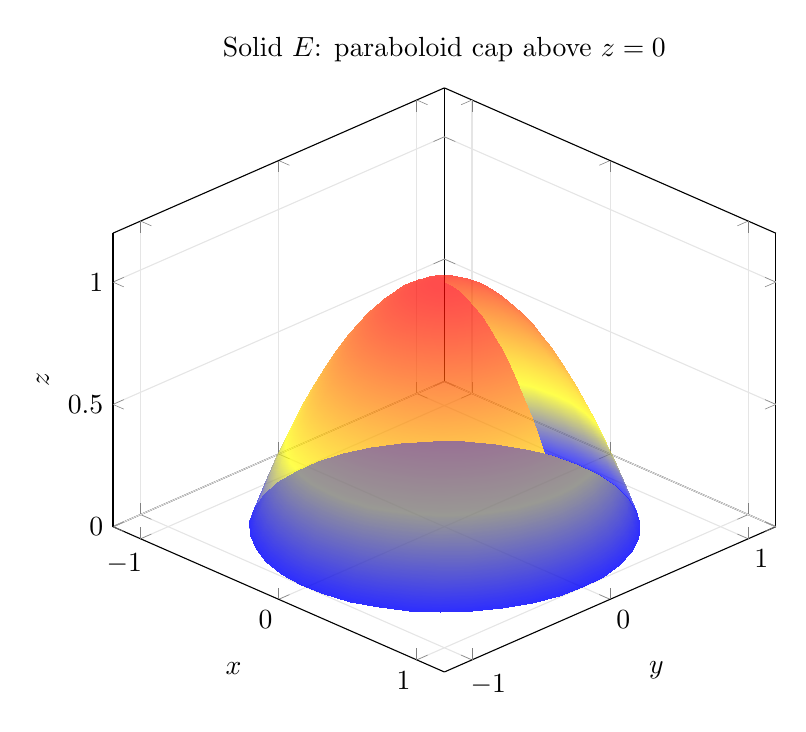
\begin{tikzpicture}
\begin{axis}[
    view={45}{35},
    xlabel={$x$}, ylabel={$y$}, zlabel={$z$},
    xmin=-1.2, xmax=1.2, ymin=-1.2, ymax=1.2, zmin=0, zmax=1.2,
    width=10cm, height=9cm,
    title={Solid $E$: paraboloid cap above $z=0$},
    grid=major, grid style={gray!20}]
\addplot3[surf, shader=interp, opacity=0.7,
    domain=0:1, y domain=0:2*pi,
    samples=20, samples y=40]
    ({x*cos(deg(y))}, {x*sin(deg(y))}, {1-x^2});
\addplot3[surf, shader=interp, opacity=0.4,
    domain=0:1, y domain=0:2*pi,
    samples=20, samples y=40, color=red]
    ({x*cos(deg(y))}, {x*sin(deg(y))}, {0});
\end{axis}
\end{tikzpicture}
\end{document}
